\section{Rekombination}\label{recombination}

Die Rekombination kreiert neue Chromosome durch eine Kombination zweier zufällig
ausgewählter bereits existierender Chromosome. Dies entspricht der normalen
Fortpflanzung in der Biologie.
Das in \emph{GEATbx} enthaltene \emph{Partially matched Crossover} Verfahren
wird im Folgenden mit dem \emph{Order Crossover} von Lawrence Davis verglichen.

% http://www.geatbx.com/docu/options-03.html
% http://citeseerx.ist.psu.edu/viewdoc/download?doi=10.1.1.61.6575&rep=rep1&type=pdf
% http://chern.ie.nthu.edu.tw/alg2003/chap-8-9.pdf
% http://siebn.de/download/GenetischeAlgorithmen.pdf

\subsection{Order Crossover (OX)}
Das von Lawrence Davis in \citep{ox} beschriebene \emph{Order Crossover} Verfahren ist nicht im
Umfang von \emph{GEATbx} enthalten und muss daher selbst implementiert werden.
Die Funktionsweise des Algorithmus wird im Folgenden schrittweise erklärt, wobei
die entsprechenden Codezeilen unserer Implementierung aus {\tt recox.m}
jeweils gelistet sind.

\newcommand{\recox}[2]{\lstinputlisting[language=Matlab, firstnumber=#1, firstline=#1, lastline=#2]{Code/recox.m}}

Die Funktion {\tt recox()} erhält die existierende Sammlung an Individuen und
die Rekombinationsrate übergeben und liefert eine neue Menge an Individuen mit
gleicher Anzahl zurück.
Die neuen Chromosomen werden mit den bisherigen initialisiert, so dass die
später nicht veränderten Individuen der Menge bereits die richtigen Werte
enthalten.

\recox{1}{5}

\noindent Neben der Länge der einzelnen Chromosomen wird deren Anzahl bestimmt.
Das erste Chromosom wird mit dem zweiten rekombiniert, das dritte mit dem vierten
und so weiter, weswegen die {\tt for}-Schleife in Zweier-Schritten über alle
Chromosome geht.
Mittels {\tt rand()} und der Rekombinationsrate wird entschieden, ob die beiden
Chromosome rekombiniert werden oder ihre alte Form behalten.

\recox{7}{13}

\noindent Zur leichteren Übersicht im weiteren Quellcode werden die beiden
Eltern-Chromosome und die beiden neuen Chromosome, welche als Kinder bezeichnet
werden, als eigene Variablen angelegt.
Sollten die beiden Eltern identisch sein, wird die weitere Berechnung
übersprungen, da die entstehenden Kinder genau den Eltern entsprechen würden.

\recox{15}{23}

\noindent Als nächstes wird per Zufall eine Start- und eine Endposition innerhalb
der Chromosomlänge gewählt, was in Abbildung \ref{fig.recox} durch die roten
gestrichelten Linien bei den Eltern dargestellt ist.
Die beiden Positionen definieren jeweils Substrings, welche an die
korrespondierende Position der Kinder-Prototypen kopiert werden.
In der grafischen Darstellung ist dies in der mittleren Reihe dargestellt, wobei
(wie im Quellcode) {\tt Child 1} den Substring von {\tt Parent 2} bekommt und
{\tt Child 2} denjenigen von {\tt Parent 1}.

\recox{25}{35}

\begin{figure}[h!]
  \centering
  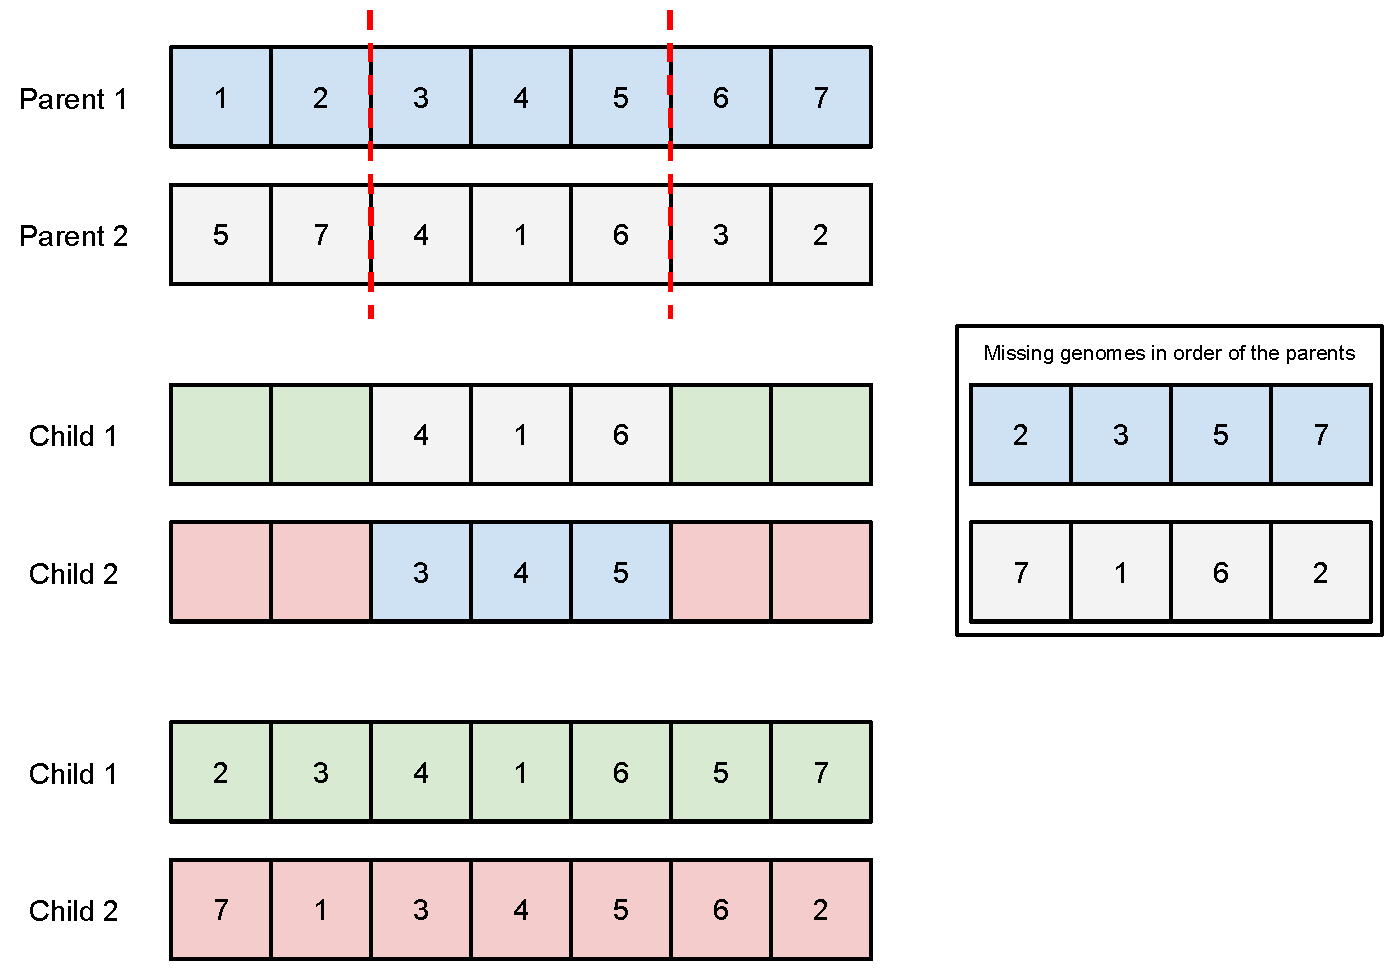
\includegraphics[width=1.0\textwidth]{Figures/recox.pdf}
  \caption{Order Crossover (OX)}\label{fig.recox}
\end{figure}

\noindent Die fehlenden Gene werden folgendermaßen aufgefüllt: Für {\tt Child 1}
wird nun eine Liste aller Gene von {\tt Parent 1} aufgebaut, welche noch nicht
in {\tt Child 1} selbst enthalten sind.
Die Reihenfolge der Gene in dieser Liste entspricht dabei der Reihenfolge wie
sie in {\tt Parent 1} auftreten. Gleiches gilt für {\tt Child 2} und
{\tt Parent 2}. Die resultierenden Genom-Listen sind auf der rechten Seite von
Abbildung \ref{fig.recox} dargestellt.

\recox{37}{41}

\noindent Die Elemente der Listen werden nun auf die noch freien Positionen der
Kinder geschrieben, wobei die Reihenfolge nicht verändert wird.
Die nun fertig rekombinierten Kinder sind im unteren Drittel der Abbildung
\ref{fig.recox} visualisiert.

\recox{43}{50}

\noindent Zuletzt werden die neu erzeugten Kinder-Chromosomen in die Menge aller
Individuen eingetragen und danach mit dem nächsten Durchlauf der Schleife
fortgefahren.

\recox{52}{57}


\subsection{Partially matched Crossover (recpm)}

Beim \emph{Partially matched Crossover} Verfahren wird auf die gleiche Weise ein
zufällig gewählter Substring in die Kinder kopiert (Abb. \ref{fig.recpm}, obere Hälfte).
An den nun noch freien Positionen übernimmt {\tt Child 1} die Gene von
{\tt Parent 1}, sofern diese nicht kollidieren, also noch nicht im Kind
enthalten sind, was im dritten Teil der Abbildung \ref{fig.recpm} dargestellt
ist.

\begin{figure}[h!]
  \centering
  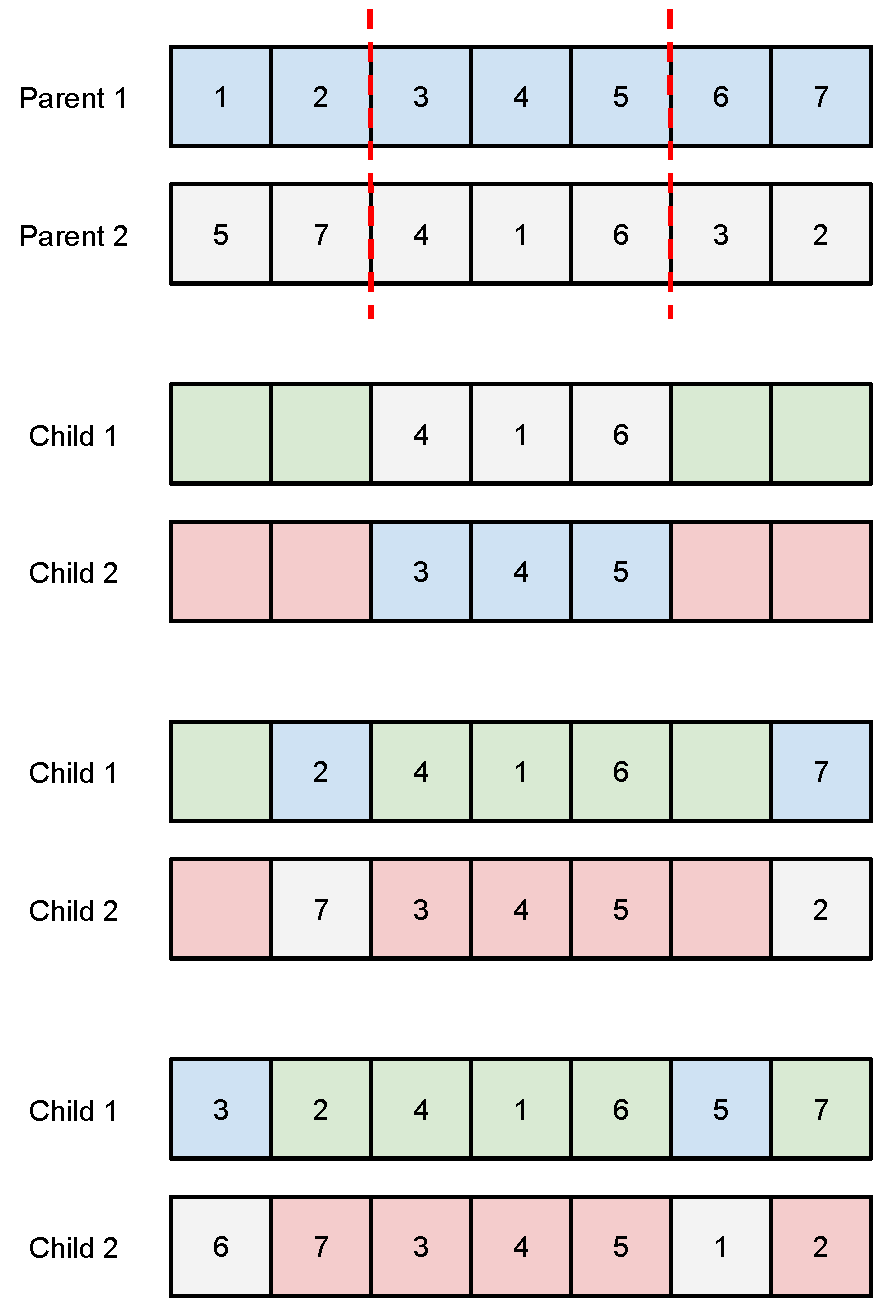
\includegraphics[width=0.7\textwidth]{Figures/recpm.pdf}
  \caption{Partially matched Crossover (recpm)}\label{fig.recpm}
\end{figure}

Die letzten fehlenden Gene werden folgendermaßen aufgefüllt: die beiden
ausgewählten Substrings definieren die Abbildung der Genome, im Beispiel der
Abbildung \ref{fig.recpm} sind dies $3 \leftrightarrow 4 \leftrightarrow 1$ und
$5 \leftrightarrow 6$.
Für das erste Gen von {\tt Child 1} wird also statt dem Wert $1$ aus der
korrespondieren Position von  {\tt Parent 1} der Wert $3$ gewählt, was im
untersten Viertel der Abbildung ersichtlich ist.
Statt dem Wert $6$ ergibt sich so für das zweitletzte Gen von {\tt Child 1}
der Wert $5$, womit das Chromosom eine gültige Form aufweist. \citep{erben}


\subsection{Ergebnisse}

Wie Tabelle \ref{Recombination.Name} zeigt, liefert \emph{Order Crossover}
(recox) mit Abstand bessere Ergebnisse.
Da das Verfahren auch die Laufzeit um ein beträchtliches Maß verringert,
fällt die Entscheidung selbstverständlich auf \emph{recox}.

\include{Chapters/gen/Recombination.Name}

